\documentclass [xcolor=svgnames, t] {beamer} 
\usepackage[utf8]{inputenc}
\usepackage{booktabs, comment} 
\usepackage[absolute, overlay]{textpos} 
\useoutertheme{infolines} 
\setbeamercolor{title in head/foot}{bg=internationalorange}
\setbeamercolor{author in head/foot}{bg=dodgerblue}
\usepackage{csquotes}
\usepackage[style=verbose-ibid,backend=bibtex]{biblatex}
\bibliography{bibfile}

\usepackage{amsmath}
\usepackage[makeroom]{cancel}

\usepackage{textpos}

\usepackage{tikz}
\usepackage{tikz-uml}
\usepackage{multirow}

\usetheme{Madrid}
\definecolor{myuniversity}{RGB}{113, 0, 0}
\definecolor{internationalorange}{RGB}{113, 0,  0}
 	\definecolor{dodgerblue}{RGB}{113, 0,0}
\usecolortheme[named=myuniversity]{structure}

\usepackage{algorithm}
\usepackage{algpseudocode}
\usepackage{caption}

\title[APT-MAC Sim. in NS-3 (MSc. Thesis)]{Simulation of a Novel MAC Protocol on the NS-3 Platform}
%\subtitle{(Introduction to Turbulence - ENGR5005G)}
\institute[]{Computer Science \\University of Rome, \\La Sapienza. }
\titlegraphic{
\includegraphics[height=2.5cm]{Sapienza_logo.jpg}}
\author[Agbeve, Douglas]{
Douglas Dziedzorm Agbeve
}


%\institute[]{Computer Science \\University of Rome, La Sapienza}
\date{March 30, 2020}


\addtobeamertemplate{navigation symbols}{}{%
    \usebeamerfont{footline}%
    \usebeamercolor[fg]{footline}%
    \hspace{1em}%
    \insertframenumber/\inserttotalframenumber
}

\begin{document}
\begin{frame}
 \titlepage   
\end{frame}




%%%%%%%%%%%%%%%%%%%%%%%%%%%%
\logo{
\includegraphics[scale=0.2]{Sapienza_logo.jpg}~%
}


%%%%%%%%%%%%%%%%%%%%%%%%%%



\begin{frame}{Outline}
\vspace{1cm}
\begin{center}
   \begin{itemize}
     \item Introduction
     \item Objectives
     \item NS-3 - An Introduction
     \item Governing Algorithm
     \item Tag-Augmented Nodes
     \item Simulation of Readers
     \item Results
     \item Conclusions and Future Work
     \item References
 \end{itemize} 
\end{center}
 
\end{frame}


\begin{frame}{Introduction }
Smart Home
 \begin{center}
\begin{columns}[onlytextwidth]
\column{0.4\textwidth}
\begin{itemize}
    \item Home appliances controlled remotely
    \item Fuelled by IoT technologies
    \item Battery usage increased in IoT era
    \item Cons of excessive battery usage
        \begin{itemize}
            \item environmental degradation
            \item stress in changing dead batteries
        \end{itemize}
\end{itemize}

\column{0.6\linewidth}
\begin{figure}
    \centering
    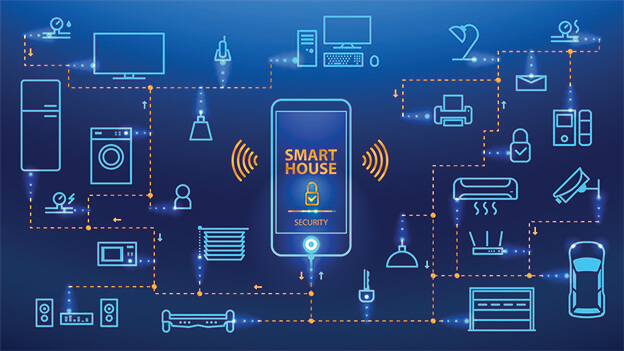
\includegraphics[width=1.0\textwidth]{smart-home-automation-2-1.jpg}
    \caption{1. Smart Home Visual (source: www.bemi.fi).}
    \label{fig:my_label}
\end{figure}

\end{columns}

\end{center}

\end{frame}

\begin{frame}{Introduction (contd...)}
    \begin{center}
        \begin{columns}[onlytextwidth]   
            \column{0.5\textwidth}
            %\vspace{1 cm}
            Battery-free Smart Home\\
            \vspace{1cm}
            \begin{itemize}
                \item  Home electronics still dependent on batteries ?
            \end{itemize}

            \column{0.5\textwidth}
            \begin{figure}
                \centering
                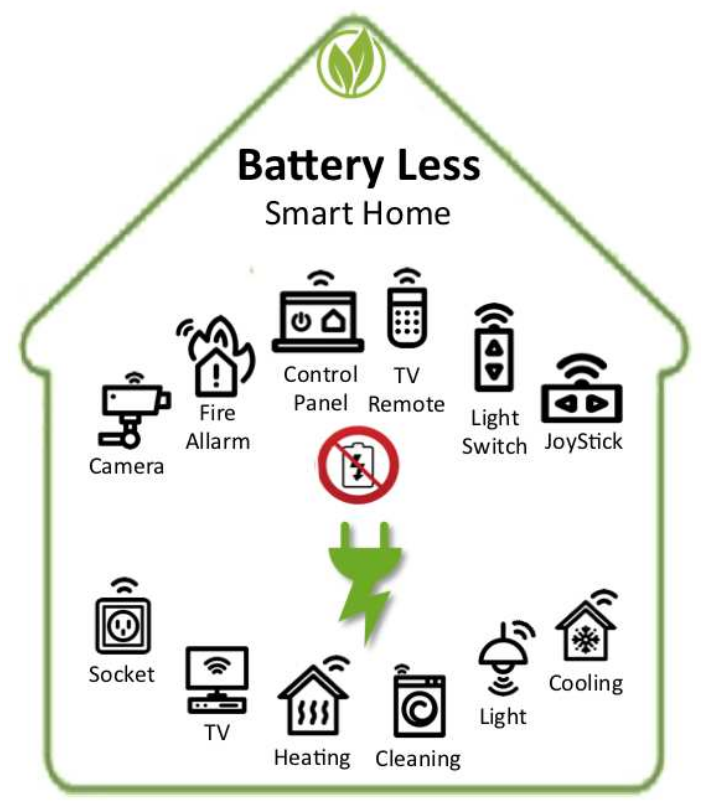
\includegraphics[width=0.65\textwidth]{not-so-smart-devices.png}
                \caption{2. Battery-free Smart Home }
                \label{fig:my_label}
            \end{figure}
        \end{columns}
    \end{center}
\end{frame}


\begin{frame}{Objectives}
    \vspace{1.5cm}   
    \begin{itemize}
        \item Introduce the NS-3 library.
        \item Understanding the Novel MAC protocol.
        \item Simulate the various battery-free home electronic devices.
        \item Simulate the Novel MAC protocol on the reader.
        \item Performance analysis of the MAC protocol.
    \end{itemize}
\end{frame}

\begin{frame}{NS-3 - An Introduction \autocite{nsonline}}
    The NS-3 Library\\
    \vspace{.5cm}
    \begin{itemize}
        \item A discrete event network simulator
        \item C$++$ and Python
        \item \textit{Waf} build system
        \item Abstractions :
            \begin{itemize}
                \item Node
                \item Application
                \item Channel
                \item Transport
                \item Network
                \item Data Link
            \end{itemize}
        \item Helpers
    \end{itemize}
\end{frame}

\begin{frame}{Governing Algorithm}
    Multi-Arm Bandit Problem\autocite{Sutton&Barto}\\
    \vspace{.5cm}
    \begin{itemize}
        \item Multiple actions with unknown reward to choose from
        \item Goal is to maximize reward margin through series of actions
        \item Example: Website advertisement to visitors
        \item Exploitation and Exploration
        \item Action-Reward function:
            \begin{equation}
                \theta^* = Q(a^*) = \mathop{\textbf{max}}_{a{\in}A}Q(a)
            \end{equation}
        \item[] Where:
            \begin{itemize}[ ]
                \item[] $Q(a_t) = \mathbb{E}[\,R | A=a]\,= \theta$
                \item[] $\theta^*$ \hspace{0.3cm} optimal probability
            \end{itemize}
   \end{itemize}
  
\end{frame}


\begin{frame}{Governing Algorithm (contd...)}
    APT-MAC Protocol\autocite{maselli}\\
    \vspace{.5cm}
    \begin{itemize}
        \item Translates into Multi-Arm Bandit as:
            \vspace{0.2cm}
            \begin{itemize}
                \item Reader: agent performing actions
                    \vspace{0.2cm}
                \item Set of Actions: query tag$_i$ , query tag$_j$ \ldots
                    \vspace{0.2cm}
                \item State set: ready to perform new query
                    \vspace{0.2cm}
                \item Computing expected reward of each action
                    \vspace{0.2cm}
                \item Keep record of the reward of each action
            \end{itemize}
    \end{itemize}

\end{frame}


\begin{frame}[allowframebreaks]{Governing Algorithm (contd...)}
    \rule{\textwidth}{0.5pt}
    \vspace*{-0.5cm}
    \captionof{algorithm}{APT-MAC pseudocode}
    \vspace*{-0.5cm}
    \rule{\textwidth}{0.5pt}
        \begin{algorithmic}[1]
            \State Master M \Comment{Reader}
            \State Set D \Comment{Devices}
            \State Map R:$(\,$d$\in$D$)\,\to$float \Comment{Reward Devices Map}
            \State Set MinQD \Comment{Minimum Query Delay}
            \State Maximum Query Delay MaxQD
            \State Set DLTH \Comment{Data Loss Threshold}
            \For{d $\in$ D}
                \State R$[\,$d$]\, = 1.0$
                \State Set MaxQD
            \EndFor
            \State R $= softmax(\,$R$)\,$
            \While{true}
                \State Device next $=$ chooseNext$(\,$R$)\,$
                \State Bool goodQuery $=$ M.query$(\,$next$)\,$
                \If{goodQuery}
                    \State R$[\,$next$]\,=$updateReward$(\,$next,bonus$)\,$
                    \If{getDataLoss $<$ DLTH}
                        \State updateMaxQD
                    \EndIf
                    \Else
                    \State R$[\,$next$]\,=$updateReward$(\,$next,malus$)\,$
                \EndIf
                \State R $= softmax(\,$R$)\,$
            \EndWhile
        \end{algorithmic}
\end{frame}


\begin{frame}{Governing Algorithm (contd...)}
    APT-MAC Protocol\\
    \vspace{.5cm}
    \begin{itemize}
        \item Reward is updated with function:
    \end{itemize}
    \begin{equation}
        Q(a_i)(n+1) = Q(a_i)(n)+\alpha(Reward - Q(a_i)(n))
    \end{equation}
    \begin{itemize}
        \item[] Where:
            \begin{itemize}
                \item[] $\alpha$\hspace{.25cm}$=$\hspace{.25cm} learning rate
            \end{itemize}
    \end{itemize}
\end{frame}

\begin{frame}{Tag-Augmented Nodes}
    Markov Representation\\
    \vspace{.5cm}
    \begin{figure}[ht]
        \begin{minipage}[b]{0.45\linewidth}
            \centering
            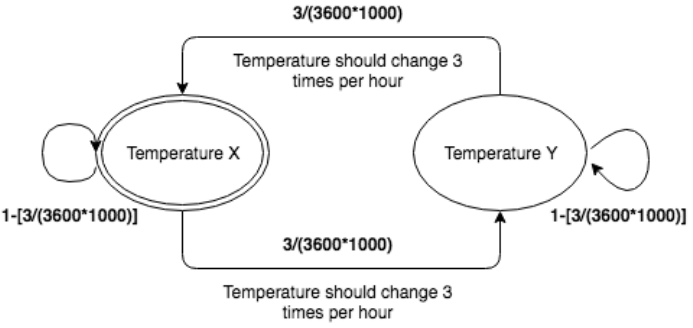
\includegraphics[width=\textwidth]{temperature-sensor}
            \caption{Temperature Sensor model}
            \label{fig:temperature-sensor}
        \end{minipage}
        \hspace{.5cm}
        \begin{minipage}[b]{0.45\linewidth}
            \centering
            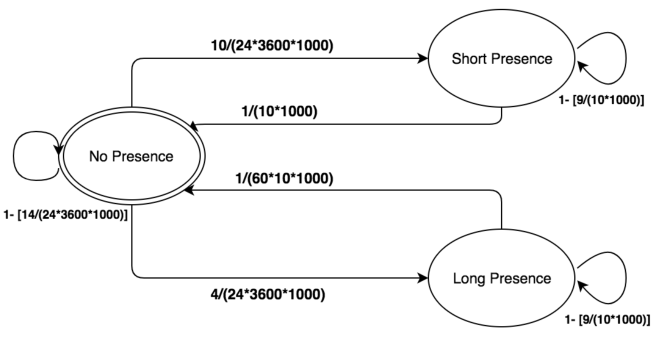
\includegraphics[width=\textwidth]{presence-sensor}
            \caption{Presence Sensor model}
            \label{fig:presence-sensor}
        \end{minipage}
    \end{figure}
   
\end{frame}


\begin{frame}{Tag-Augmented Nodes (contd...)}
    Markov Representation\\
        \vspace{.5cm}
        \begin{figure}[ht]
            \begin{minipage}[b]{0.45\linewidth}
             \centering
                 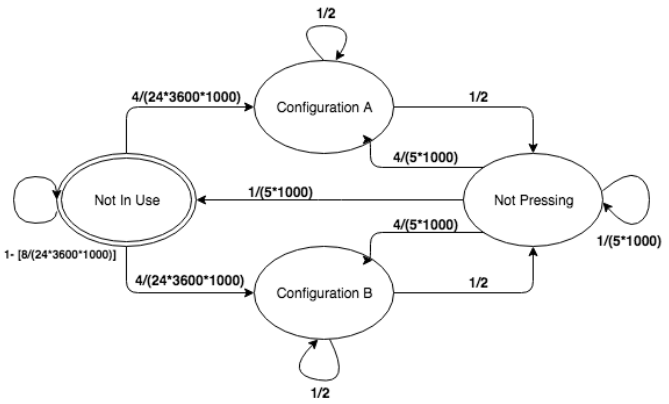
\includegraphics[width=\textwidth]{tv-remote}
                 \caption{TV Remote model}
                 \label{fig:tv-remote}
             \end{minipage}
             \hspace{.5cm}
             \begin{minipage}[b]{0.45\linewidth}
                 \centering
                 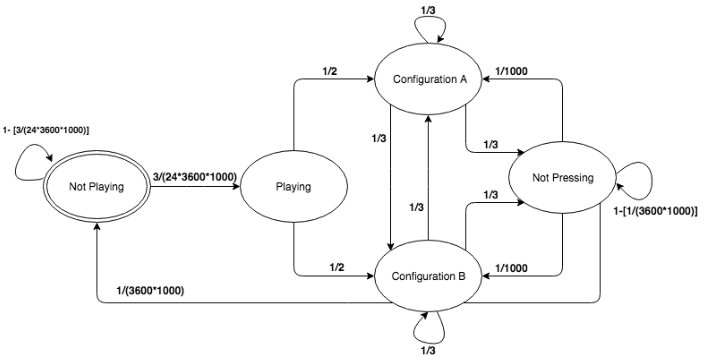
\includegraphics[width=\textwidth]{joysick-sensor}
                 \caption{Joystick model}
                 \label{fig:joysick-sensor}
             \end{minipage}
         \end{figure}

\end{frame}

\begin{frame}{Tag-Augmented Nodes (contd...)}
    Packet Header\\
    \begin{figure}
        \begin{tikzpicture}[scale=0.85]
            \tikzumlset{font=\tiny\ttfamily}
            \umlemptyclass[x=0,y=0]{Header}{
                }{}
\umlclass[x=5.5,y=-2]{AptMacHeader}{
  -m\_id : uint16\_t \\ -m\_type : uint16\_t \\ -m\_stateChange : uint16\_t \\ 
  -m\_dataLoss : uint16\_t
}{
  +AptMacHeader() \\ +SetId(id : uint16\_t) : void \\ +GetId (void) : const
  uint16\_t\\ +SetPacketType(ptype : uint16\_t) : void \\ +GetPacketType(void) :
  const uint16\_t \\ +SetStateChange(stateChange : uint16\_t) : void \\ 
  +GetStateChange(void) : const uint16\_t \\ \umlstatic{+GetTypeId(void) : TypeId} 
  \\ +GetDataLoss(void) : const uint16\_t \\ +SetDataLoss(d : uint16\_t) : void \\
  \umlvirt{+Serialize(start : Buffer::Iterator) : const void} \\
  \umlvirt{+Deserialize(start : Buffer::Iterator) : uint32\_t} \\
  \umlvirt{+GetSerializedSize(void) : const uint32\_t} \\
  \umlvirt{+GetInstanceTypeId (void) : const TypeId} \\
  \umlvirt{+Print(\&os : std::ostream) : const void}\\
}
\umlenum[x=11.5,y=-4]{HeaderContents}{
    BROADCAST : uint16\_t \\ DATA : uint16\_t \\ STATECHANGE : uint16\_t
}

\umlaggreg[geometry=-|]{AptMacHeader}{HeaderContents}
\umlinherit[geometry=-|]{AptMacHeader}{Header}
\end{tikzpicture}
\caption{Class Diagram - APT-MAC Header}
\label{fig:headerUML}
    \end{figure}
\end{frame}


\begin{frame}{Tag-Augmented Nodes (contd...)}
    Devices Simulation\\
    \begin{figure}
        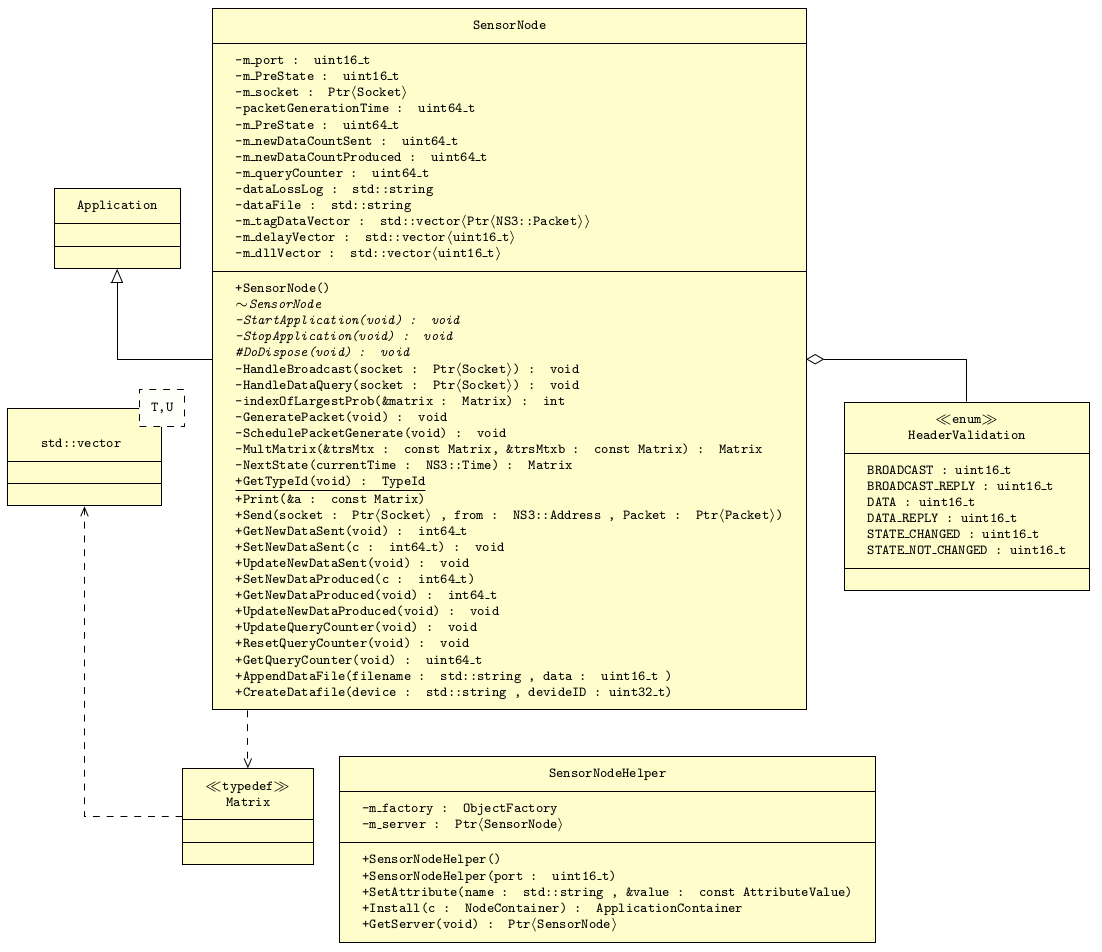
\includegraphics[width=.75\textwidth,height=.75\textheight]{sensory-node-class-diagram}
        \captionof{figure}{Class Diagram - Sensory Nodes}
        \label{fig_nodeUML}
    \end{figure}

\end{frame}


\begin{frame}{Tag-Augmented Nodes (contd...)}
    Devices Simulation\\
    \vspace{.5cm}
    \begin{itemize}
        \item Enumeration of some functions :
            \begin{itemize}
                \item StartApplication
                \item StopApplication
                \item HandleBroadcast
                \item HandleDataQuery
                \item GeneratePacket
                \item SchedulePacketGenerate
                \item NextState
                \item Send
                \item UpdateNewDataSent
                \item UpdateNewDataProduced
                \item GetQueryCounter
            \end{itemize}
    \end{itemize}
       
\end{frame}

\begin{frame}{Simulation of Readers}
    APT-MAC Reader\\
    \vspace{.5cm}
    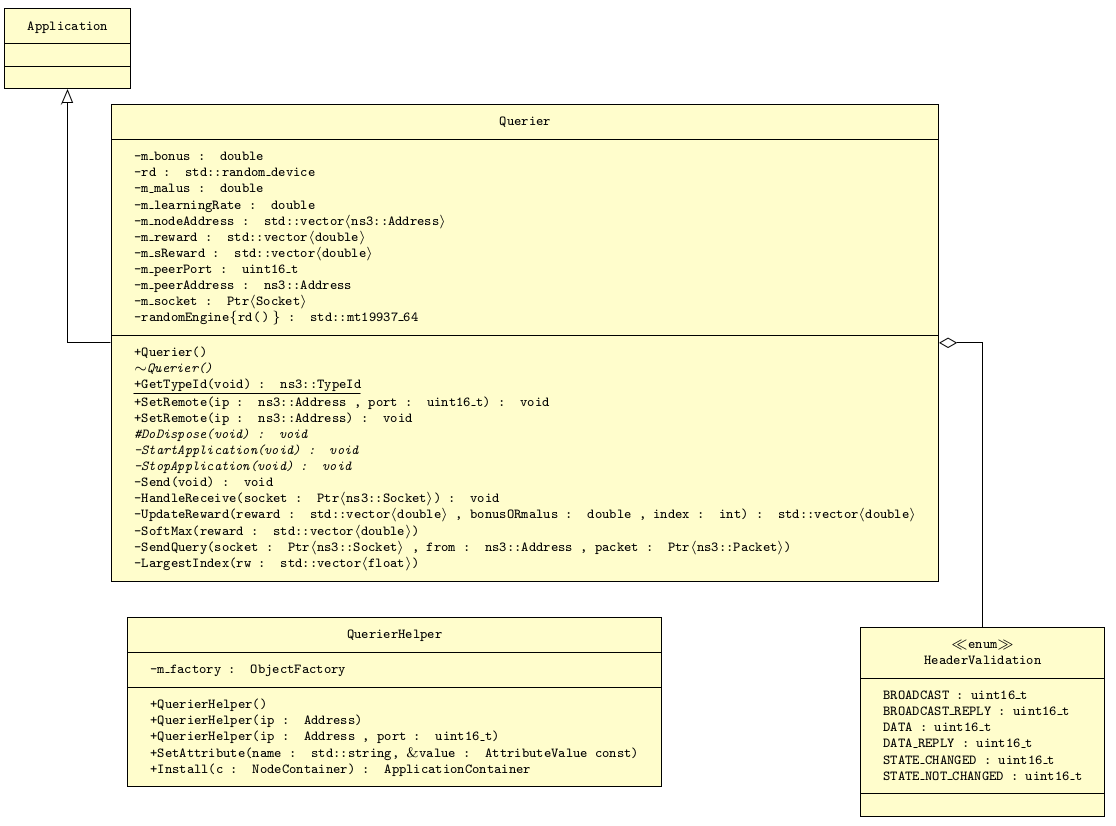
\includegraphics[width=.75\textwidth,height=.75\textheight]{querrier-class-diagram}
    \captionof{figure}{Class Diagram - APT-MAC Reader}
    \label{fig_apt-mac-readerUML}

\end{frame}



\begin{frame}{Simulation of Readers (contd\ldots)}
    TDMA Reader\\
    \vspace{.5cm}
    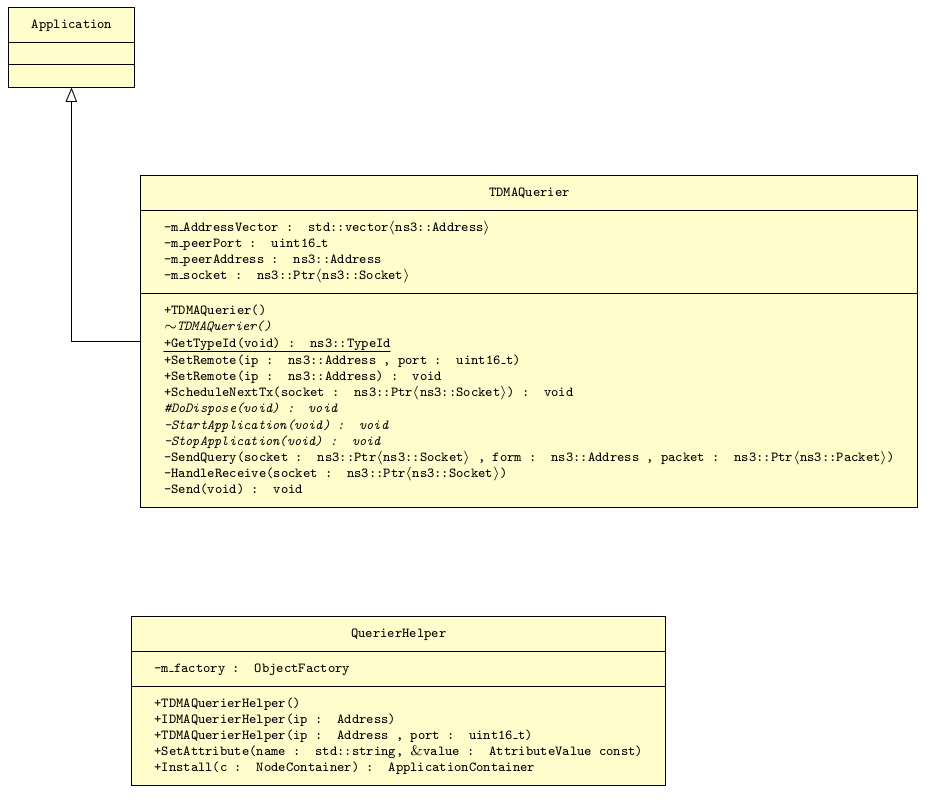
\includegraphics[width=.75\textwidth,height=.75\textheight]{tdma-class-diagram}
    \captionof{figure}{Class Diagram - APT-MAC Reader}
    \label{fig_apt-mac-readerUML}
\end{frame}


\begin{frame}{Simulation of Readers (contd\ldots)}
    Run Configuration.\\
    \vspace{.5cm}
    \begin{itemize}
        \item Data rate of the net-device and channel set to 640\textit{kbps}.
        \item Tag memory 256 bits
    \end{itemize}
\end{frame}


\begin{frame}{Results}
    Performance Metrics\\
    \vspace{.5cm}
    \begin{itemize}
        \item Packet Delay :
            \begin{itemize}
                \item[] the difference in time between generating a packet data and sending to the reader.
            \end{itemize}
        \item Data Loss :
            \begin{itemize}
                \item[] this is the percentage of generated data that is not delivered to the reader.
            \end{itemize}
    \end{itemize}
\end{frame}

\begin{frame}{Results (contd\ldots)}
    \begin{table}[h!]
    \caption{WORKLOAD SCENARIOS DESCRIPTION}
    \label{tab:WSD}
    \centering
    \begin{tabular} { | c | c | c | c | c | }
        \hline
        \multicolumn{1}{| c }{No. of Sensors}  & \multicolumn{1}{c }{Scenario}
                                             & \multicolumn{1}{ c }{Joystick}
                                             & \multicolumn{1}{ c }{Remote}
                                             & \multicolumn{1}{ c |}{Env. Sensors} \\
        \hline
        \hline
        \multirow{4}{*}{20} & Case 1 & 1 & 2 & 17 \\ 
                            & Case 2 & 2 & 3 & 15 \\ 
                            & Case 3 & 3 & 3 & 14 \\ 
                            & Case 4 & 4 & 4 & 12 \\
        \hline
        \multirow{4}{*}{30} & Case 1 & 1 & 2 & 27 \\
                            & Case 2 & 2 & 3 & 25 \\
                            & Case 3 & 3 & 3 & 24 \\
                            & Case 4 & 4 & 4 & 22 \\
        \hline
        \multirow{4}{*}{40} & Case 1 & 1 & 2 & 37 \\
                            & Case 2 & 2 & 3 & 35 \\
                            & Case 3 & 3 & 3 & 34 \\
                            & Case 4 & 4 & 4 & 32 \\
        \hline
    \end{tabular}
\end{table}
\end{frame}

\begin{frame}{Results (contd\ldots)}
    Transient time :
    \begin{itemize}
        \item[] duration for APT-MAC device to get into optimum performance of reduced data loss.
    \end{itemize}
    \begin{figure}
        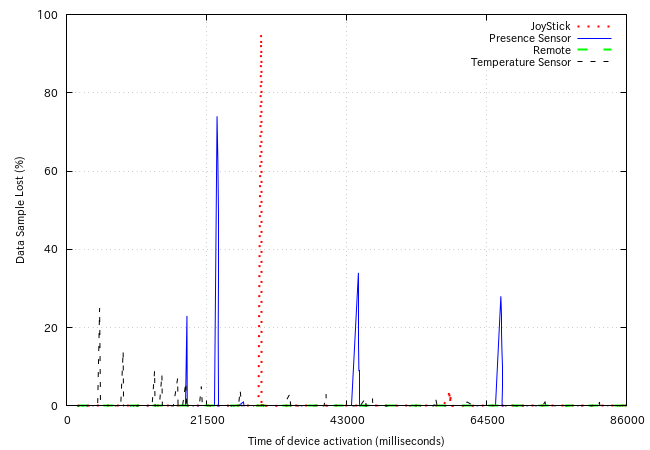
\includegraphics[width=.7\textwidth,height=.6\textheight]{transcient}
        \caption{Transient Time}
    \end{figure}
\end{frame}


\begin{frame}{Results (contd\ldots)}
    Transient time\\
    \vspace{.5cm}
    \begin{itemize}
        \item approximately 50\textit{ms} to get the data loss of a joystick to less than 15\%
        \item 0.283\textit{s} for presence sensor
        \item temperature sensor took approximately a milli of a second.
    \end{itemize}
\end{frame}

\begin{frame}{Results (contd\ldots)}
    Performance based on uptime - 20 Devices
    \vspace{.5cm}
    \begin{figure}[ht]
        \begin{minipage}[b]{0.48\linewidth}
             \centering
                 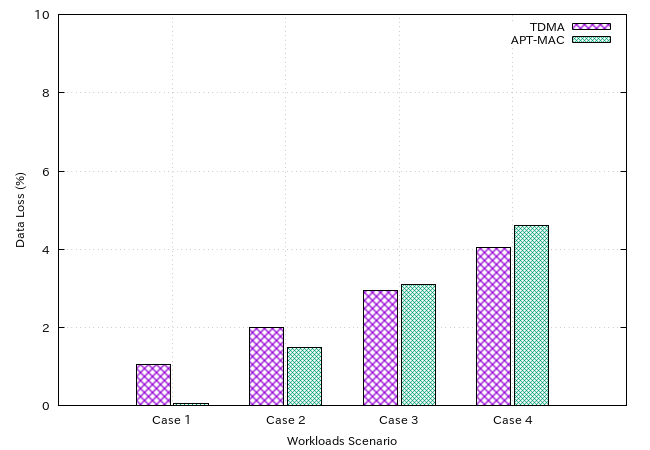
\includegraphics[width=\textwidth]{20-1-data-loss-short-period}
                  \caption{Data Loss Short Run}
                   \label{fig:20-device-short-run}
                 \end{minipage}
                 \hspace{.2cm}
                 \begin{minipage}[b]{0.48\linewidth}
                     \centering
                     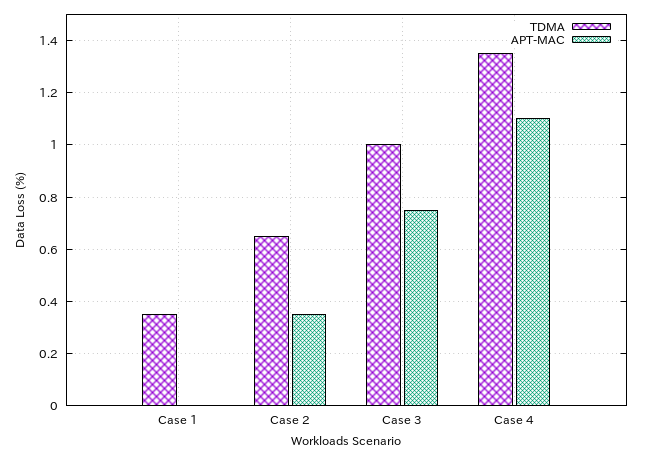
\includegraphics[width=\textwidth]{20-1-data-loss}
                     \caption{Data Loss}  
                     \label{fig:fig:20-device-DL}
                 \end{minipage}
             \end{figure}
\end{frame}

\begin{frame}{Results (contd\ldots)}
    \begin{figure}[ht]
        \centering
        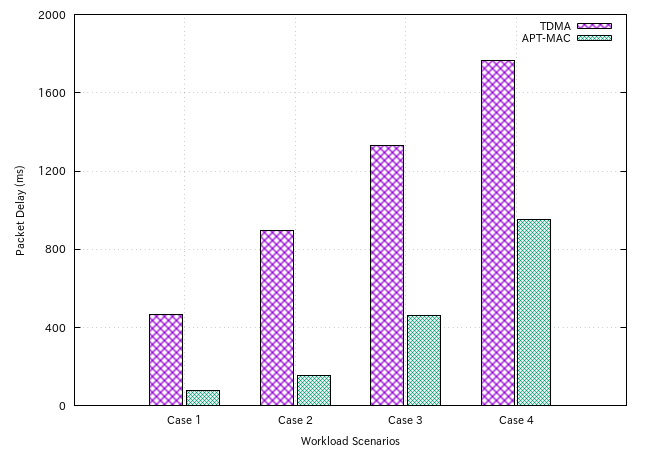
\includegraphics[width=.8\textwidth,height=.7\textheight]{20-1-packet-delay}
        \caption{20 Devices : Packet Delay}
        \label{fig:20-devices-PD}
    \end{figure}

\end{frame}

\begin{frame}{Results (contd\ldots)}
    \vspace{.5cm}
    \begin{figure}[ht]
        \begin{minipage}[b]{0.48\linewidth}
             \centering
                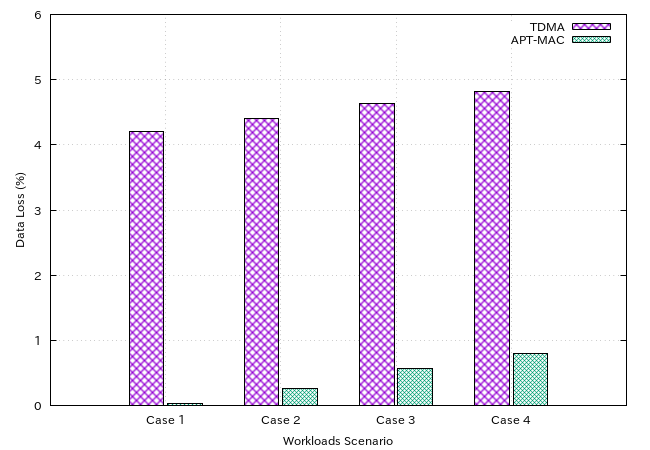
\includegraphics[width=\textwidth]{30-data-loss}
                \caption{30 Devices : Data Loss}
                \label{fig:30-device-dl}
        \end{minipage}
                     \hspace{.2cm} 
                     \begin{minipage}[b]{0.48\linewidth}
                         \centering
                         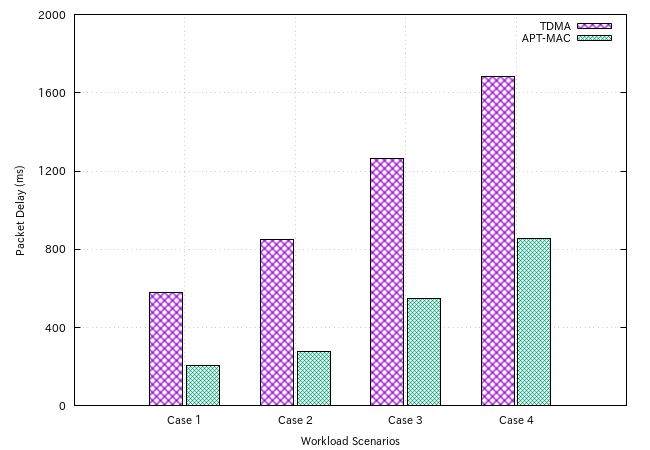
\includegraphics[width=\textwidth]{30-packet-delay}
                         \caption{30 Devices : Packet Delay}  
                         \label{fig:fig:30-device-PD}
        \end{minipage}
    \end{figure}
\end{frame}


\begin{frame}{Results (contd\ldots)}
       \vspace{.5cm}
         \begin{figure}[ht]      
             \begin{minipage}[b]{0.48\linewidth}
                \centering
                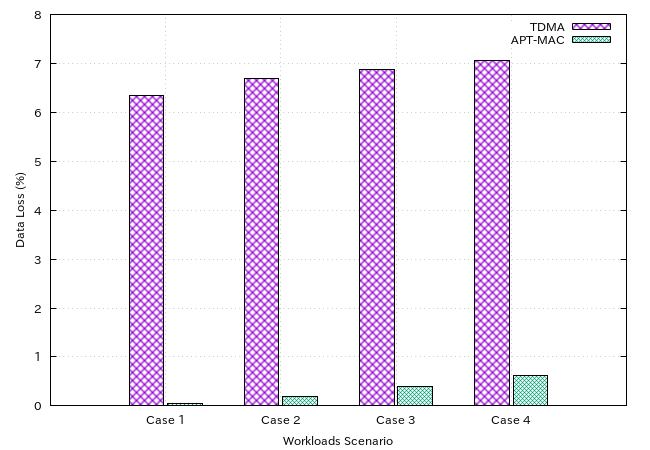
\includegraphics[width=\textwidth]{40-data-loss}
                 \caption{40 Devices : Data Loss}          
                 \label{fig:40-device-dl}                  
         \end{minipage}                                    
                      \hspace{.2cm} 
                      \begin{minipage}[b]{0.48\linewidth}
                          \centering
                          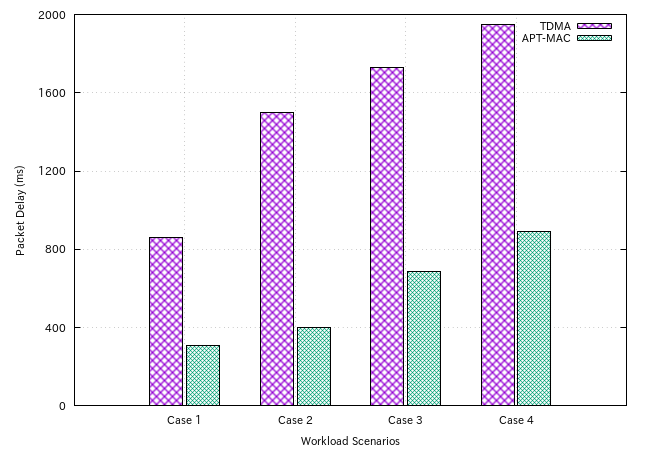
\includegraphics[width=\textwidth]{40-packet-delay}
                          \caption{40 Devices : Packet Delay}          
                          \label{fig:fig:40-device-PD}                     
                       \end{minipage}                                      
                   \end{figure}                                            
\end{frame}



\begin{frame}{Conclusions and Future Work}
    \textbf{Conclusion}
    \begin{itemize}
        \item Objectives met
        \item APT-MAC outperforms TDMA
    \end{itemize}
    \textbf{Future Work}
    \begin{itemize}
        \item Mobility of the devices with respect to APT-MAC
        \item other variants of reinforcement algorithms
    \end{itemize}
\end{frame}
\begin{frame}{References}
   \printbibliography
\end{frame}

\end{document}
